\documentclass[a4paper,11pt]{article}
\usepackage{amsmath,amssymb,graphicx,hyperref}
\usepackage[margin=0.85in]{geometry}

\usepackage{tocloft} % For custom table of contents
\usepackage{xcolor}  % For link and text color
\usepackage{subcaption}% multiple graphs side by side
\usepackage{booktabs} %these two makes tables look better
\usepackage{tabularx}
\usepackage{doi}
\usepackage{url}
\usepackage{cite}
\usepackage{xcolor}
\usepackage{dsfont}
\usepackage{slashed}
\usepackage{minted}
\usepackage{leftindex}
\usepackage{physics}


\definecolor{LightGray}{gray}{0.9}
% Set link colors
\hypersetup{
	colorlinks=true,
	linktoc=page,      % Makes only page numbers clickable
	linkcolor=blue,    % Link color (e.g., for TOC)
	urlcolor=cyan,     % URL link color
	citecolor=magenta  % Citation link color
}


\title{\textbf{Partonic and Hadronic Cross-section Calculations for $pp \rightarrow W^+ \rightarrow e^+ \nu_e$}}

\author{
	Edwin Varghese\\[10pt]
	\small Department of Physics, Royal Holloway, University of London, Egham Hill, TW20 0EX, U.K.\\
	\texttt{\small zkap069@live.rhul.ac.uk}
}

\date{}

\begin{document}
	
	\maketitle
	
	\begin{abstract}
	
		
		
	\end{abstract}
	
	
	\newpage
	\tableofcontents

\section{$u\bar{d} \rightarrow W^+$ cross-section derivation}
\subsection{Obtaining the partonic cross-section $\hat{\sigma}(u\bar{d} \rightarrow W^+)$}
Generally, calculating tree-level amplitudes of electroweak interactions involve two or more spinors contracted with each other by boson propagators. After writing down the Feynman diagram corresponding to the interaction, one uses the Feynman rules to formulate an amplitude, $\mathcal{M}$, which is used in the analytical expression for the cross-section with an appropriate spin and/or colour sum or average.\\

The interaction that is of interest is the hadronic production of $W \rightarrow e \nu $. To predict $W \rightarrow e \nu$ distributions, one must calculate the complete production and decay subprocesses, $$u \bar{d} \rightarrow W^+ \rightarrow e^+ \nu_e.$$ To start, the cross-section for a simple $u \bar{d} \rightarrow W^+$ is derived below.
\begin{figure}[h]
	\centering
	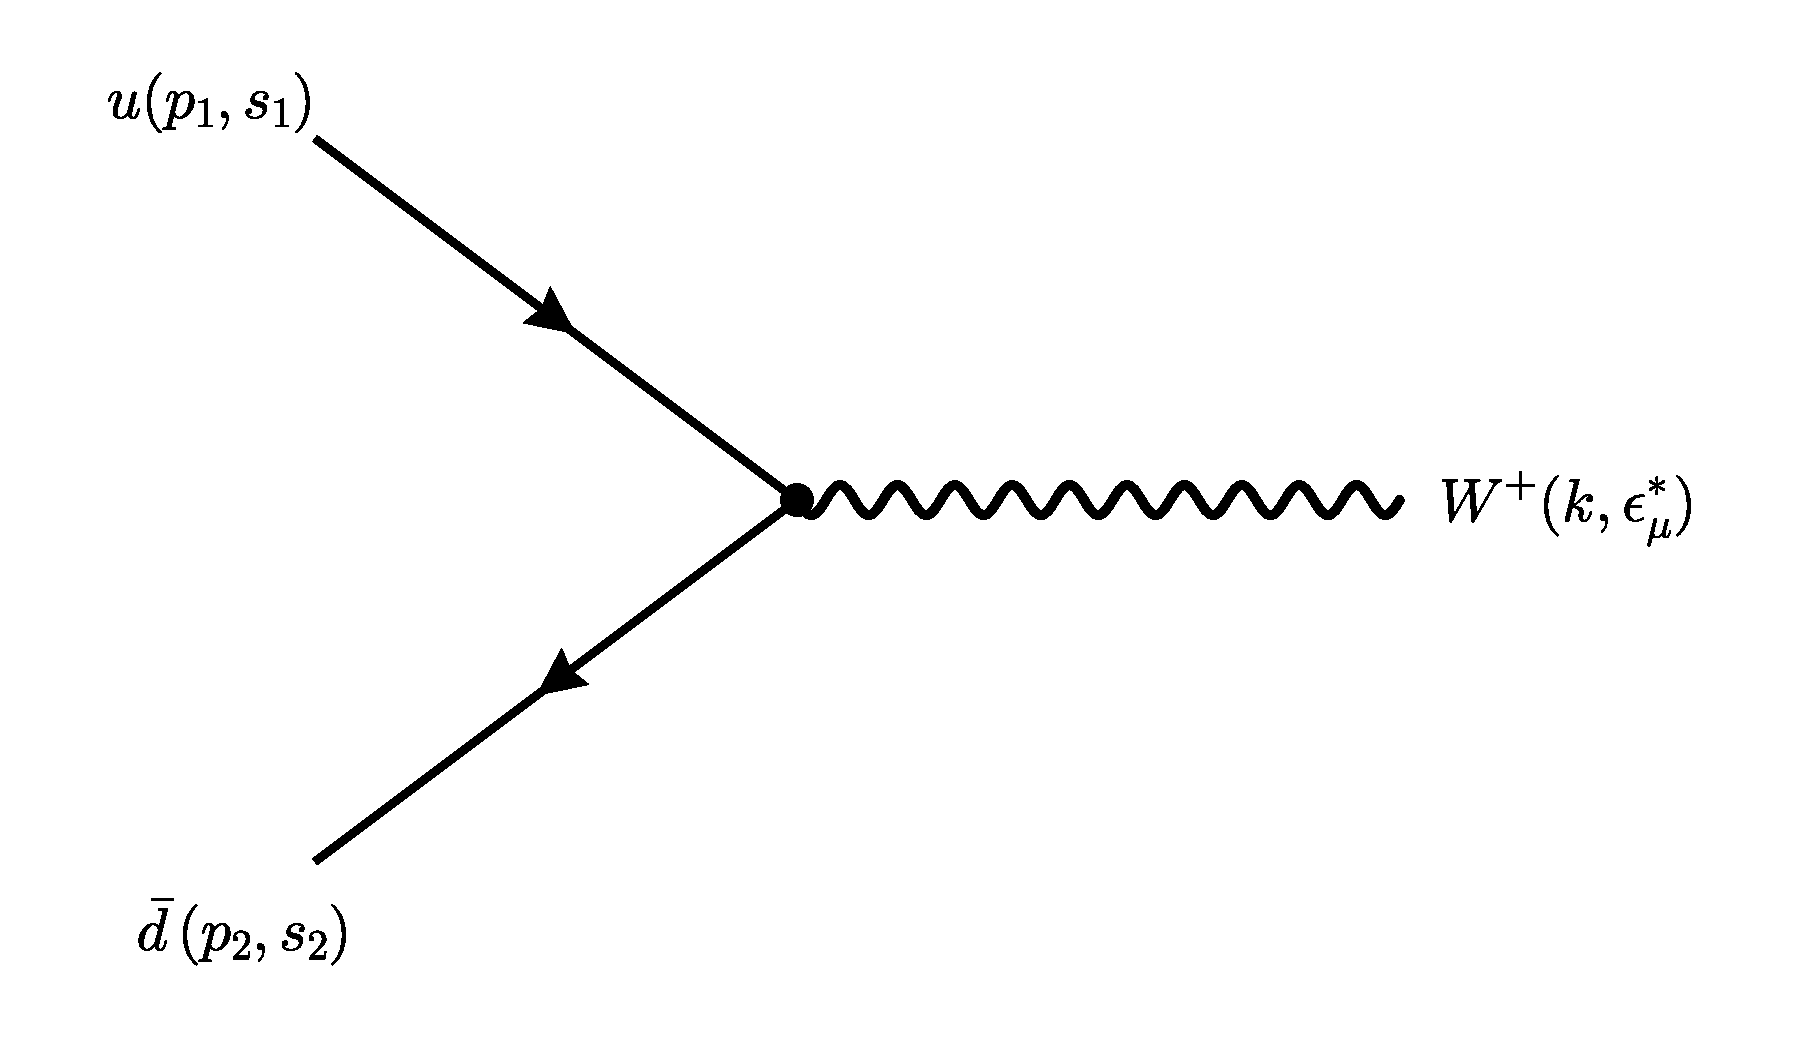
\includegraphics[width=0.7\linewidth]{graphics/u-antid-wplus_v3}
	\caption{Feynman diagram representing the annihilation of an up quark with an anti-down quark, creating a $W^+$ boson.}
\end{figure}


\underline{Feyman Rules}:
\begin{itemize}
	\item Following the fermion line backwards, anti-down-quark is represented as a Dirac $\bar{v}$-spinor, where the bar corresponds to a four-component row vector, with four-momentum $p_2$, mass $m_2$ and spin $s_2$.
	\item In this case, W$^+$ is not a propagator, but an external spin-1 particle, thus is represented as the vector boson current, $$-i\frac{g}{\sqrt{2}}\frac{1}{2}\gamma^\mu (1-\gamma^5)\text{V}_\text{ud}\epsilon_\mu^*(k, \lambda),$$ and one includes the polarisation vector, $\epsilon_\mu^*(k, \lambda)$, where $\lambda = 0, \pm1$ corresponds to the longitudinal and two transverse polarisation states of the W-boson and the momentum four-vector $k  = p_1 +p_2$. The factor $\text{V}_\text{ud}$ is an element of the CKM matrix, and represents a complex amplitude that quantifies the strength of the weak coupling between the up-quark weak eigenstate to the down-quark mass eigenstate. $|\text{V}_\text{ud}|^2$ is the probability that an up-quark transitions to a down-quark via weak interaction, and is approximated to be 1, thus we omit writing it in the amplitude. The factor of $\frac{1}{2}$, is due to the fact that the charged weak interaction only couples to left-chiral fermions (and right-chiral anti-fermions).
	\item  The fermion line ends at the up-quark, which is represented as a Dirac u-spinor, which corresponds to a four-component column vector, with four-momentum $p_1$, mass $m_1$ and spin $s_1$.
\end{itemize}	
 The amplitude, $\mathcal{M}$, is therefore: $$\mathcal{M} = \bar{v}(p_2, s_2) 	\left[-i\frac{g}{\sqrt{2}}\frac{1}{2}\gamma^\mu (1-\gamma^5) \right] u(p_1, s_2) \epsilon_\mu^{*}(k, \lambda).$$ Squaring the amplitude gives: $$ |\mathcal{M}|^2= |\mathcal{M}^*\mathcal{M}| = \frac{1}{4} \frac{g^2}{2} \left(\bar{v}(p_2, s_2)\gamma^\mu (1-\gamma^5) u(p_1, s_1) \epsilon_\mu^* \right)^* \left(\bar{v}(p_2, s_2)\gamma^\nu (1-\gamma^5) u(p_1, s_1) \epsilon_\nu^*(k, \lambda) \right).$$ The complex conjugated term is a scalar, thus, can be written equivalently as the term conjugate transposed,
 
  $$ \left(\bar{v}(p_2, s_2)\gamma^\mu (1-\gamma^5) u(p_1,  s_1) \epsilon_\mu^*(k, \lambda) \right)^* \equiv \left(\bar{v}(p_2, s_2)\gamma^\mu (1-\gamma^5) u(p_1, s_1) \epsilon_\mu^*(k, \lambda) \right)^\dagger. $$ Using the relation, $\bar{v}=v^\dagger \gamma^0$, 
  $$ \left(v^\dagger(p_2, s_2)\gamma^0 \gamma^\mu (1-\gamma^5) u(p_1, s_1) \epsilon_\mu^*(k, \lambda) \right)^\dagger.$$
  
  From here on, the brackets indicating the four-momentum and spin of the quarks and the momentum four-vector and polarisation vector of the W will be omitted; using the reverse-order law, $(ABC)^\dagger = C^\dagger B^\dagger A^\dagger$ where A,B, C are matrices, and $\gamma^{0 \dagger} = \gamma^0$,  one gets:
 \begin{equation}\label{gamma_id}
 	\begin{aligned}
 		 	\epsilon_\mu u^\dagger \left[\gamma^\mu (1-\gamma^5)\right]^\dagger \gamma^0 v &= \epsilon_\mu u^\dagger \gamma^0 \gamma^0 \left[\gamma^\mu (1-\gamma^5)\right]^\dagger \gamma^0 v \\
 		&= \epsilon_\mu \bar{u}[\overline{\gamma^\mu (1-\gamma^5)}] v.
 	\end{aligned}
 \end{equation}

 
 On the second line, a factor of $\gamma^0 \gamma^0 = \mathds{1}_4$, was introduced so that the identity, $\bar{\Gamma}= \gamma^0 \Gamma^\dagger \gamma^0$, where $\Gamma = \gamma^\mu (1-\gamma^5)$, can be used. The $\bar{u}=u^\dagger \gamma^0$ was also used. The squared amplitude now looks like:
 
 \begin{equation}\label{msquared}
 	|\mathcal{M}|^2 = \frac{1}{4} \frac{g^2}{2} (\epsilon_\mu \bar{u}[\overline{\gamma^\mu (1-\gamma^5)}]v)(\bar{v}[\gamma^\nu (1-\gamma^5] u \epsilon_\nu^*).
 \end{equation}
 
 \subsubsection{Summing over quark spin states}\label{completeness}
 When $|\mathcal{M}|^2 $ is summed over the possible values of the spin indices, $s_1$ and $s_2$, terms like $\sum_{s_1} \bar{u}u$ and $\sum_{s_2} \bar{v}v$ will appear; these can be evaluated using the completeness relation for Dirac spinors: %can add proof of completeness realtions using lecture notes
 \begin{itemize}
 	\item $\sum_{s}u\bar{u} =  \slashed{p}+m  $
 	\item $\sum_{s}v\bar{v} =  \slashed{p}-m  $
 \end{itemize}
 Note that $\epsilon_{\mu}$ and $\epsilon_{\nu}^*$ will be treated separately later (i.e. the polarisations will be summed over) and will not contribute in the summation over spins. The notation for spin- and polarisation-summed amplitude squared will then split into the summation over spins component, denoted by $S^{\mu\nu}$, and summation over polarisation, denoted $P_{\mu \nu}$, where, $$\sum_{s_1, s_2, \text{pol}}|\mathcal{M}|^2=  \frac{1}{4} \frac{g^2}{2}P_{\mu\nu}S^{\mu\nu} $$\\
 
  Start off by summing over the spins of the $\bar{d}$-quark (i.e. using the Dirac v-spinor completeness relation). 
 
\begin{equation}\label{msquared_spin2}
	S^{\mu\nu}= \bar{u} [\overline{\gamma^\mu (1-\gamma^5)}] (\slashed{p_2}-m_2) [\gamma^\nu (1-\gamma^5)] u.
\end{equation}  
In order to sum over the spins of the up-quark (i.e. the Dirac u-spinor), let $\Lambda=   [\overline{\gamma^\mu (1-\gamma^5)}] (\slashed{p}-m) [\gamma^\nu (1-\gamma^5]$; Eq. (\ref{msquared_spin2}) becomes:

\begin{equation}\label{msquared_spin2_2}
	S^{\mu\nu}= (\bar{u}\Lambda u).
\end{equation}  

The matrix multiplication $(\bar{u}\Lambda u)$ can be written in component form as 
$$(\bar{u}\Lambda u)= \sum_{a,b=1}^4 (\bar{u})_a (\Lambda)_{ab} (u)_b = \sum_{a,b=1}^4 (\Lambda)_{ab} (u)_b(\bar{u})_a = \sum_{a,b=1}^4 (\Lambda)_{ab} (u\bar{u})_{ba} \sum_{a= 1}^4 = [\Lambda u\bar{u}]_{aa} = \text{Tr}[\Lambda u \bar{u}].$$ Summing over $s_1$ gives 

$$ \bar{u}\Lambda u = \sum_{s_1} \text{Tr}[\Lambda u \bar{u}] = \text{Tr}[\Lambda(\slashed{p}_1+m_1)].$$ Unpacking $\Lambda$ gives the end result $$S^{\mu\nu}= \text{Tr}\left[\overline{\gamma^\mu (1-\gamma^5)} (\slashed{p}_2-m_2) \gamma^\nu (1-\gamma^5)(\slashed{p}_1+m_1)\right].$$ This procedure is known as Casimir's trick which replace the sum over spin states with the spinor completeness relations, in order to turn products of spinors into a trace over gamma matrices that one can evaluate with standard trace identities. Since the $\bar{\Gamma}= \gamma^0 \Gamma^\dagger \gamma^0$ identity was used to soak up two of the $\gamma^0$s in Eq.(\ref{gamma_id}), it can be shown that,

\begin{equation}\label{overline-id}
	\begin{aligned}
		\overline{\gamma^\mu (1-\gamma^5)} &= \gamma^0 [\gamma^\mu(1-\gamma^5)]^\dagger \gamma^0 \\
		&= \gamma^0(1-\gamma^5)\gamma^{\mu \dagger}\gamma^0 \\
		&= \gamma^0(1-\gamma^5)\gamma^0 \gamma^\mu \gamma^0 \gamma^0 \\
		&= \gamma^\mu (1-\gamma^5),
	\end{aligned}
\end{equation}
where $(\gamma^5)^\dagger = \gamma^5$, $(\gamma^\mu)^\dagger = \gamma^0  \gamma^\mu \gamma^0$, and $\{\gamma^5, \gamma^\mu\}= 0$ was used. This gives,
\begin{equation}\label{M_s}
	S^{\mu\nu}= \text{Tr}\left[\gamma^\mu (1-\gamma^5)(\slashed{p}_2-m_2)\gamma^\nu (1-\gamma^5)(   \slashed{p}_1+m_1) \right].
\end{equation}

One can use the projector representation of $(1-\gamma^5)$ and its properties to simplify this expression. The left-handed chirality projection operator is defined as $P_L = \frac{1}{2}(1-\gamma^5)$ and the right-handed chirality projection operator is defined as $(1+\gamma^5)$; Eq.(\ref{M_s}) in this representation becomes,

$$2\text{Tr}\left[\gamma^\mu P_L (\slashed{p}_2-m_2)\gamma^\nu P_L (\slashed{p}_1+m_1) \right].$$ 

 Moving a factor of $(1- \gamma^5)$ through $\gamma^\mu$ results in a minus sign, since $\{\gamma^5, \gamma^\mu\}=0$, so $(1 - \gamma^5)\gamma^\mu = \gamma^\mu(1+ \gamma^5)$. In the projector representation one has $P_L \gamma^\mu =\gamma^\mu P_R$, which is entirely equivalent. One gets,
 
 $$2\text{Tr}\left[\gamma^\mu P_L (\slashed{p}_2-m_2)P_R\gamma^\nu(\slashed{p}_1+m_1) \right].$$ 

Applying $P_L$ and $P_R$ on the left and right hand side of $(\slashed{p}_2-m_2)$ respectively gives,

$$P_L\slashed{p}_2 P_R - P_L m_2 P_R = P_L \gamma^\sigma p_{2\sigma} P_R - P_L m_2 P_R $$

The factors $m_2$ and $p_{2\sigma}$ commute with the projection operators, thus, the $P_R$ in the first term can be moved next to $\gamma^\sigma$ and $P_R$ can be moved next to the $P_L$,
$$P_L \gamma^\sigma P_R p_{2\sigma} - P_LP_R m_2,$$ 
and then using the $P_L \gamma^\mu =\gamma^\mu P_R$ relation, one gets,

$$P_L^2 \gamma^\sigma p_{2\sigma} - P_LP_R m_2.$$

Since $P_L^2 = P_L$ and $P_LP_R=0$, this reduces to,

$$P_L \gamma^\sigma p_{2\sigma} = P_L \slashed{p}_2 = (1-\gamma^5)\slashed{p}_2.$$
Since the labels $1$ and $2$ that were chosen for $u$ and $\bar{d}$ respectively were arbitrary, one can make the argument that the coefficient of the $m_1$ term will also go to zero. The trace is therefore,

 $$2\text{Tr}\left[\gamma^\mu P_L \slashed{p}_2\gamma^\nu\slashed{p}_1 \right]= 2\text{Tr}\left[\gamma^\mu (1-\gamma^5) \slashed{p}_2\gamma^\nu\slashed{p}_1\right] $$ 
Essentially, the amplitude squared --- and thus the cross-section --- of the $u \bar{d} \rightarrow W^+$ process is independent of the masses of the quarks.


\begin{equation}\label{traces1}
	\begin{aligned}
		S^{\mu\nu} &= 2\text{Tr}\left[\gamma^\mu (1-\gamma^5)\slashed{p}_2\gamma^\nu \slashed{p}_1\right] \\
		&=  2\text{Tr}\left[\gamma^\mu \slashed{p}_2\gamma^\nu \slashed{p}_1 \right] - 2\text{Tr}\left[ \gamma^\mu \gamma^5 \slashed{p}_2\gamma^\nu \slashed{p}_1 \right]
	\end{aligned}
\end{equation}

One can now use the trace identities to evaluate Eq.(\ref{traces1}).\\
Using, $ \text{Tr}[\slashed{p}\gamma^\mu \slashed{k} \gamma^\nu] = 4[p^\mu k^\nu + p^\nu k^\mu - (p \cdot k) g^{\mu \nu}]$ on the first term and $\text{Tr}[\gamma^\mu \gamma^\nu \gamma^\rho \gamma^\sigma \gamma^5] = -4i\epsilon^{\mu \nu \rho \sigma}$, where $\epsilon_{\mu \nu \rho \sigma}$ is the totally anti-symmetric Levi-Civita symbol, on the second gives,

\begin{equation}\label{traces_first_term}
	\begin{aligned}
		2\text{Tr}\left[\gamma^\mu \slashed{p}_2\gamma^\nu \slashed{p}_1 \right] = 8[p_2^\mu p_1^\nu + p_2^\nu p_1^\mu - (p_1 \cdot p_2) g^{\mu \nu}]
	\end{aligned}
\end{equation}
\begin{equation}\label{traces_second_term}
	\begin{aligned}
	2\text{Tr}\left[ \gamma^\mu \gamma^5 \slashed{p}_2\gamma^\nu \slashed{p}_1 \right] &=   	2\text{Tr}\left[ \gamma^\mu \gamma^5  \gamma^\rho p_{1\rho} \gamma^\nu \gamma^\sigma p_{2\sigma} \right]\\ 
	&= 2p_{1\rho}p_{2\sigma}\text{Tr}\left[ \gamma^\mu \gamma^5 \gamma^\rho \gamma^\nu \gamma^\sigma \right]= 2p_{1\rho}p_{2\sigma}\text{Tr}\left[ \gamma^\mu \gamma^\rho \gamma^\nu \gamma^\sigma \gamma^5 \right] \\
	&=  2p_{1\rho}p_{2\sigma} (-4i \epsilon^{\mu \rho\nu\sigma})\\
	&= 8i \epsilon^{\mu \nu \rho \sigma}p_{1\rho}p_{2\sigma}.
	\end{aligned}
\end{equation}
$p_{1\rho}$ and $p_{2 \sigma}$ are components of 4-momenta for the up-quark and anti-down-quark respectively, and can be taken out of the trace (i.e. the trace of a scalar is the scalar itself). The cyclicity of traces (Tr$[ABC]=$Tr$[ABC]=$Tr$[ABC]$, where $ABC$ are matrices) was used on the second line to move $\gamma^5$ the right most side of the trace. The $\rho$ index was switched with the $\nu$ index, in the third line to the fourth line, producing a minus sign that cancels with the pre-existing minus. The spin-summed squared amplitude becomes, $$S^{\mu\nu}= 8[p_2^\mu p_1^\nu + p_2^\nu p_1^\mu - (p_1 \cdot p_2) g^{\mu \nu} -i \epsilon^{\mu \nu \rho \sigma}p_{1\rho}p_{2\sigma}].$$ 

\subsubsection{Summing over final polarisation states}\label{pol}
As mentioned earlier, the W$^{+}$ is an external particle in the $u\bar{d} \rightarrow W^+$ process. A W boson has two transverse and on longitudinal polarisation, and the cross section must include the contribution of every polarisation state, thus must be summed over. For a massive W boson with momentum $p^\mu$ and mass $M_W$, summing over polarisation states gives,

\begin{equation}
	P_{\mu\nu}= \sum_\text{pol} \epsilon_\mu \epsilon_\nu^*=  -g_{\mu\nu} + \frac{k_\mu k_\nu}{M_W^2},
\end{equation}
where $k$ is the four-momentum of the external W boson. The spin- and  polarisation-summed squared amplitude gives,

\begin{equation}\label{spin_pol_square_amp}
	\sum_{s_1, s_2, \text{pol}} |\mathcal{M}|^2=  \frac{1}{4} \frac{g^2}{2} P_{\mu\nu}S^{\mu\nu}= \frac{1}{4} \frac{g^2}{2} \left(-g_{\mu\nu} + \frac{k_\mu k_\nu}{M_W^2}\right)8[p_2^\mu p_1^\nu + p_2^\nu p_1^\mu - (p_1 \cdot p_2) g^{\mu \nu} - i \epsilon^{\mu \nu \rho \sigma}p_{1\rho}p_{2\sigma}].
\end{equation}
This expression needs to be evaluated by contracting the indices. Contracting the $g_{\mu\nu}$ with the terms in the square brackets gives,
\begin{equation}
	\begin{aligned}
		-8[p_{2\mu}p_1^\mu + p_{1\mu}p_2^\mu -4(p_1 \cdot p_2) -ig_{\mu\nu}\epsilon^{\mu \nu \rho \sigma}p_{1\rho}p_{2\sigma}] &= 8[-2(p_1 \cdot p_2) + 4(p_1 \cdot p_2)- 0] \\
		&= 16(p_1 \cdot p_2).
	\end{aligned}
\end{equation}
 The contraction of $g_{\mu\nu}\epsilon^{\mu \nu \rho \sigma}p_{1\rho}p_{2\sigma}$ goes to zero because the Levi-Civita is totally antisymmetric and the metric tensor is symmetric under the exchange of indices, i.e. exchanging the $\mu$ and $\nu$ indicies gives,
 
 $$g_{\mu\nu} = g_{\nu\mu} \; \text{and}\; \epsilon_{\mu \nu \rho \sigma} = - \epsilon_{\nu \mu \rho \sigma},$$ 
 and so, 
 $$ g_{\mu\nu}\epsilon^{\mu \nu \rho \sigma}p_{1\rho}p_{2\sigma} = - g_{\nu\mu}\epsilon^{\nu \mu \rho \sigma}p_{1\rho}p_{2\sigma}= 0 \qquad \forall \rho,\sigma. $$
  The factor of 4 comes from the contraction $g_{\mu\nu}g^{\mu\nu}$. Contracting $\frac{k_\mu k_\nu}{M_W^2}$ gives,
 
 \begin{equation}\label{k}
 	\begin{aligned}
		\frac{8}{M_W^2}[2(p_2 \cdot k)(p_1 \cdot k ) - k^2 (p_1 \cdot p_2)+ k_\mu k_\nu (\epsilon^{\mu \nu \rho \sigma}p_{1\rho}p_{2\sigma})] &=  \frac{8}{M_W^2}[2(p_2 \cdot k)(p_1 \cdot k ) - k^2 (p_1 \cdot p_2)+ 0] 
 	\end{aligned}
 \end{equation}
Similarly, the $k_\mu k_\nu (\epsilon^{\mu \nu \rho \sigma}p_{1\rho}p_{2\sigma})$ goes to zero, for all $\rho$ and $\sigma$, due to $k_\mu k_\nu$ being totally symmetric under exchange of indicies and the Levi-Civita being totally antisymmetric under the exchange of indicies. Momentum has to be conserved, so one can assume that $k = p_1 + p_2$, which corresponds to saying that the W$^+$ boson carries the momentum of both up and anti-down quarks, and thus $k^2 = ( p_1 + p_2)^2 = p_1^2 + p_2^2 +2p_1\cdot p_2$. Assuming massless quarks, $p^2 = E^2 - |p|^2 = 0 $, so $k^2 = 2p_1\cdotp_2$. Substituting back into Eq. \ref{k} gives,

$$\frac{8}{M_W^2}[2(p_1 + p_2) \cdot p_2 (p_1 +p_2 )\cdot p_1 - (2p_1\cdot p_2)(p_1 \cdot p_2)]  = \frac{8}{M_W^2}[2(p_1 \cdot p_2)^2 - 2(p_1 \cdot p_2)^2] = 0.$$	
Therefore the contraction with $g_{\mu\nu}$ is the only term that survives, given the massless fermion approximation. The spin- and  polarisation-summed amplitude squared gives,


\begin{equation}\label{spin_pol_square_amp2}
	\sum_{s_1, s_2, \text{pol}} |\mathcal{M}|^2= \frac{1}{4} \frac{g^2}{2}16(p_1 \cdot p_2)
\end{equation}

\subsubsection{Spin and colour averages}
For an unpolarised beam, the initial spin is not known and so one must average over all possible spin states. The incoming up quark and anti-down quark each can have spin +$\frac{1}{2}$ or $-\frac{1}{2}$, thus, the average is $\frac{1}{4}$. In the same manner, one averages over initial colour states by dividing by the number of initial colour states.  The up and anti-down quark each have three possible colour states, ($r$,$g$,$b$) and ($\bar{r}$,$\bar{g}$,$\bar{b}$) respectively. The naive colour averaged factor is $\frac{1}{9}$. Since, the weak interaction is a colour singlet, a red quark can only annihilate with an anti-red, green with anti-green, and blue with anti-blue. The initial colour degree of freedom is reduced to 3 and the colour averaged factor is now $\frac{1}{3}$. One can express the amplitude in terms of the mass of the W boson, $M_W$, via the relation between the weak coupling constant, $g$, and the Fermi constant, $G_F$,

$$G_F = \frac{\sqrt{2} g^2}{8M_W^2}$$. One can then express the amplitude as,


$$\sum_{s_1, s_2, \text{pol}} |\mathcal{M}|^2=  \frac{G_F}{\sqrt{2}} M_W^2 \left(\frac{1}{4}\right)_{\text{spin}}\left(\frac{1}{3}\right)_{\text{colour}}16(p_1 \cdot p_2)  =  \frac{G_F}{\sqrt{2}} M_W^2 \frac{4}{3}(p_1 \cdot p_2) $$

Finally the $(p_1 \cdot p_2)$ term can be expressed in terms of the Mandelstam variable, $\hat{s}$; this is useful since $\sqrt{\hat{s}}$ is equivalent to the centre of mass energy of the up-anti-down pair, which is a measurable quantity. In the massless quark approximation,  $\hat{s} = (p_1+p_2)^2 = 2p_1 \cdot p_2$, thus, 

\begin{equation}\label{amp}
	\sum_{s_1, s_2, \text{pol}} |\mathcal{M}|^2= \frac{\sqrt{2}}{3}G_F M_W^2 \hat{s}
\end{equation}

\subsubsection{Cross-section formula derivation}
One can think of the initial quarks as wave-packets that can evolve with time and overlap with wave-packets representing a desired set of final-state particles. This will lead to a probability amplitude for producing that final state, which can be related to the cross-section. One can define a time-independent creation operator for a particle with momentum around $\boldsymbol{k}_i$ as

\begin{equation}\label{creation op}
	\hat{w}_{\boldsymbol{k}_i}^\dagger = \int \frac{d^3\boldsymbol{k}}{(2\pi)^2}\frac{1}{\sqrt{E_{\boldsymbol{k}}}}  f(\boldsymbol{k})\hat{a}_{\boldsymbol{k}}^\dagger,
\end{equation}
where $\hat{a}_{\boldsymbol{k}}^\dagger$ is the momentum-mode creation operator that appears in the quantised field mode expansion of the free scalar field

 $$\hat{\psi}(\boldsymbol{x},t) = \int \frac{d^3 \boldsymbol{k}}{(2\pi)^2}\frac{1}{\sqrt{2E_k}}(\hat{a}_{\boldsymbol{k}}e^{-i(p\cdot x)} + \hat{a}_{\boldsymbol{k}}^\dagger e^{i(p\cdot x)}).$$

$\hat{a}_{\boldsymbol{k}}^\dagger \ket{0}$ creates a one-particle momentum eigenstate $\ket{\boldsymbol{k}}$ that, under time-evolution and with  $\boldsymbol{k} \neq 0$, propagates and is delocalised in space due to the field mode expansion being a plane-wave solution of the Klein-Gordon equation. Naturally, this makes it non-normalisable, but introducing a function $f(\boldsymbol{k})$ that smears the wave-packet in momentum space which gives it a finite width, so that, $\bra{0}\hat{w}_{\boldsymbol{k}_i}\hat{w}_{\boldsymbol{k}_i}^\dagger\ket{0}=1.$ One can take the form of $f(\boldsymbol{k})$ to be Gaussian. One creates a localised wavepacket from a vacumm by applying Eq.(\ref{creation op}) to the state $\ket{0}$,

$$\hat{w}_{\boldsymbol{k}_i}^\dagger\ket{0} = \int \frac{d^3 k}{(2\pi)^3}\frac{1}{\sqrt{2E_k}}\phi(\boldsymbol{k})\ket{\boldsymbol{k}} = \ket{\phi}. $$

The factor of $\sqrt{2E_{\boldsymbol{k}}}$ fixes the normalisation such that,
\begin{equation}\label{normalisation}
	\bra{\phi}\ket{\phi} = 1 \qquad \text{if} \qquad \int\frac{d^3k}{(2\pi)^3}|\phi(\boldsymbol{k})|^2 = 1
\end{equation} 
	The probability is then, 

$$\mathcal{P} = |\bra{\phi_1 \phi_2 ...}\ket{\phi_A \phi_B}|^2$$
for a two incoming wave-packet states $\ket{\phi_A \phi_B}$ and for all possible outgoing wave-packet states $\bra{\phi_1 \phi_2 ...}$. One can imagine the uniformly distributed wave-packets $\phi_B(\boldsymbol{k}_B)$ being incident on the $\phi_A(\boldsymbol{k}_A)$, some wave-packets are not directly incident on $\phi_A(\boldsymbol{k}_A)$ in position space as they are shifted perpendicular to the direction of motion by a vector $\boldsymbol{b}$, called the impact parameter, in position space. To account for this one adds a factor of $e^{-i\boldsymbol{b}\cdot \boldsymbol{k}_b}$ to its momentum-space amplitude. One can write the initial state as

\begin{equation}\label{in_states}
	\ket{\phi_A\phi_B}_\text{in} = \int \frac{d^3k_A}{(2\pi)^3} \int \frac{d^3k_B}{(2\pi)^3} \frac{\phi_A(\boldsymbol{k}_A)}{\sqrt{2E_A}}\frac{\phi_B(\boldsymbol{k}_B)e^{-i\boldsymbol{b}\cdot \boldsymbol{k}_b}}{\sqrt{2E_B}} \ket{\boldsymbol{k}_A\boldsymbol{k_B}}_\text{in}.
\end{equation}


If one sets up $\ket{\phi_A \phi_B}$ such that the wave-packets $\phi_i (\boldsymbol{k})$ become concentrated about definite momenta $\boldsymbol{k}_i$, this defines an "in" state, $\ket{\boldsymbol{k}_A\boldsymbol{k}_B}_\text{in}$.

One can also define the final/out state as

$$\leftindex_{\text{out}}{\bra{\phi_1\phi_2...}} = \left(\prod_{f} \int\frac{d^3p_f}{(2\pi)^3} \frac{\phi_f(\boldsymbol{p}_f)}{\sqrt{2E_f}}\right)\leftindex_{\text{out}}{\bra{\boldsymbol{p}_1\boldsymbol{p}_2...}}. $$

The transition amplitude from the initial wave-packet to a particular final multi-particle state is given by

$$\leftindex_{\text{out}}{\bra{\phi_1\phi_2...}}S\ket{\phi_A\phi_B}_\text{in}$$

where $S$ is the S-matrix. If the particles do not interact, then S is the identity matrix; the part of the S-matrix that is of interest is the part due to interactions, which one can isolate by defining the T-matrix as
$$S = \mathds{1} + iT.$$

$S$ or $T$ must obey 4-momentum conservation, so must contain a factor of $\delta^4(k_A + k_B - \Sigma p_f)$ to enforce this. One can define the invariant amplitude as,

\begin{equation}\label{momentum-enforce}
	\bra{\boldsymbol{p}_1 \boldsymbol{p}_2 ...}iT\ket{\boldsymbol{k}_A\boldsymbol{k}_B}_\text{in} = (2\pi)^4 \delta^4(k_A + k_B - \Sigma p_f) \cdot i\mathcal{M}(k_A, k_B \rightarrow p_f)
\end{equation}


The expression for the probability for initial state particles A and B to scatter and produce a final state of n particles is given as, 

\begin{equation}\label{probability}
	\mathcal{P}(A,B \rightarrow 1, 2, ..., n)= \left(\prod_{f} \frac{d^3p_f}{(2\pi)^3} \frac{\phi_f(\boldsymbol{p}_f)}{\sqrt{2E_f}}\right)  |\leftindex_{\text{out}}{\bra{\boldsymbol{p}_1 \boldsymbol{p}_2 ...}}\ket{\phi_A\phi_B}_\text{in}|^2.
\end{equation}				


The number of scattering events N is given by,

$$N = \sum_{\text{incident particles,i}} \mathcal{P}_i = \int d^2b\; n_B \mathcal{P}(\boldsymbol{b}),$$
where  $n_b$ is the number density of particles --- number of $B$ particles per unit area --- and $\mathcal{P}(\boldsymbol{b})$ is the probability that particle B with impact parameters $\boldsymbol{b}$ will scatter off the target A. Assuming that $n_B$ is constant, it can be factored out the integral and moved to the left-hand side, 

\begin{equation}\label{nb}
	\frac{N}{n_B} =\int d^2b\; \mathcal{P}(\boldsymbol{b}) 
\end{equation}
Eq.(\ref{nb}) has dimensions of Area$^{2}$, and is equivalently the cross-section, $\sigma.$ One can now combine equations (\ref{nb}), (\ref{probability}), (\ref{in_states}) to get an expression for $d\sigma$,

\begin{gather*}
		d\sigma = \left(\prod_{f} \frac{d^3p_f}{(2\pi)^3} \frac{\phi_f(\boldsymbol{p}_f)}{\sqrt{2E_f}}\right) 
		\int d^2b \left(  \int \frac{d^3k_A}{(2\pi)^3}\frac{\phi_A(\boldsymbol{k}_A)}{\sqrt{2E_A}} \int  \frac{d^3k_B}{(2\pi)^3}\frac{\phi_A(\boldsymbol{k}_B)}{\sqrt{2E_B}} \int \frac{d^3\overline{k_A}}{(2\pi)^3} \frac{\phi^*_A(\overline{\boldsymbol{k}}_A)}{\sqrt{2\overline{E_A}}}\			\int \frac{d^3\overline{k_B}}{(2\pi)^3}\frac{\phi_B(\overline{\boldsymbol{k}}_B)}{\sqrt{2E_B}}\right)\\ 			
		\cross e^{i\boldsymbol{b}\cdot(\overline{\boldsymbol{k}}_B - \boldsymbol{k}_B)}	\left|\bra{\boldsymbol{p}_f}\ket{\boldsymbol{k}_A}\right|^2 \; \left|\bra{\boldsymbol{p}_f}\ket{\boldsymbol{k}_B}\right|^2,
\end{gather*}
which can be written compactly as,
\begin{equation}
	\begin{gathered}\label{final}
		d\sigma = \left(\prod_{f} \frac{d^3p_f}{(2\pi)^3} \frac{\phi_f(\boldsymbol{p}_f)}{\sqrt{2E_f}}\right) 
		\int \left(\prod_{i =A,B} \int \frac{d^3k_i}{(2\pi)^3}\frac{\phi_i(\boldsymbol{k}_i)}{\sqrt{2E_i}} \int  \frac{d^3\overline{k_i}}{(2\pi)^3}\frac{\phi^*_i(\overline{\boldsymbol{k}_i})}{\sqrt{2\overline{E_i}}}\right) \\
		\cross e^{i\boldsymbol{b}\cdot(\overline{\boldsymbol{k}}_B - \boldsymbol{k}_B)} \bra{\boldsymbol{p}_i}\ket{\boldsymbol{k}_i}\; \bra{\boldsymbol{p}_f}\ket{\overline{\boldsymbol{k}_i}}^*. 
	\end{gathered}
\end{equation}


The $d^2b$ integral can be preformed on the phase factor of $e^{i\boldsymbol{b}\cdot(\overline{\boldsymbol{k}}_B - \boldsymbol{k}_B)}$ to give a factor of $(2\pi)^2\delta^2(\boldsymbol{k}_B - \overline{\boldsymbol{k}_B})$. The final two factors can be written in terms of $\mathcal{M}$ using Eq.(\ref{momentum-enforce}):
 
\begin{gather*}
	\bra{\boldsymbol{p}_i}\ket{\boldsymbol{k}_i} = (2\pi)^4 \delta^4(\Sigma k_i - \Sigma p_f) \cdot i\mathcal{M}(k_i \rightarrow p_f)\\
	\bra{\boldsymbol{p}_f}\ket{\overline{\boldsymbol{k}_i}}^* = (2\pi)^4 \delta^4(\Sigma \overline{k_i} - \Sigma p_f) \cdot (-i\mathcal{M^*}(\overline{k_i}\rightarrow p_f)).	
\end{gather*}
The six $\overline{k}$ integrals can be performed using the second of these delta functions and $(2\pi)^2\delta^2(\boldsymbol{k}_B - \overline{\boldsymbol{k}_B})$. As mentioned before, the initial wave-packets are localised momentum space around $\boldsymbol{p}_A$ and $\boldsymbol{p}_B$. This means one can evaluate functions $\phi_A(\boldsymbol{k}_A)$ and  $\phi_B(\boldsymbol{k}_B)$ at $\boldsymbol{p}_A$ and $\boldsymbol{p}_B$. Eq.(\ref{final}) becomes,

\begin{gather*}
		d\sigma = \left(\prod_{f} \frac{d^3p_f}{(2\pi)^3} \frac{\phi_f(\boldsymbol{p}_f)}{\sqrt{2E_f}}\right)  \frac{|\mathcal{M}(p_Ap_B \rightarrow p_f)|^2}{2E_A2E_B|v_A-v_B|}\int \frac{d^3k_A}{(2\pi)^3}\int \frac{d^3k_B}{(2\pi)^3} \\
		\cross |\phi_A(\boldsymbol{k}_A)|^2\;|\phi_B(\boldsymbol{k_B})|^2 (2\pi)^4 \delta^4(k_A +k_B -\Sigma p_f)
\end{gather*}
Particle detectors have finite resolution; they partition momentum space into finite-size bins and register which bin the particle fell into. Due to this, the detector cannot tell apart the slight variations in momenta within each bin of the initial wave-packets $\phi_A$ and $\phi_B$, and so one can approximate the momentum $k_A + k_B$ inside the delta function at $\boldsymbol{p}_A + \boldsymbol{p}_B$. Applying the normalisation condition from (\ref{normalisation}), gives the final form of the differential cross-section:

\begin{equation}\label{general_cross}
	d\sigma  =\frac{|\mathcal{M}|^2}{2E_A 2E_B |v_A - v_B|}d\Phi_{n_f}.
\end{equation}

The factor $d\Phi_{n_f}$ is the Lorentz invariant phase space factor and is defined as,
$$d\Phi_{n_f} = (2\pi)^4 \delta^4(p_A +p_B - \Sigma p_f) \prod_{f}^{N_f}\frac{d^3\boldsymbol{p}_f}{(2\pi)^32E_f},$$

where A, B are the inital state particles and $N_f$ are the number of final state particles. Phase space refers to the subspace of the $3N_f$-dimensional momentum space of the final state particles that satisfy total energy and momentum conservation; this is enforces through the $\delta^4(p_A +p_B - \Sigma p_f)$ term. In this case, the only final state particle is the W$^+$ boson thus, $N_f =1$, and the initial particles A, B are the up and anti-down quark respectively and so the phase space factor reduces to,

\begin{equation}\label{LIPS}
	d\Phi_{1} = (2\pi)^4 \delta^4(p_u +p_{\bar{d}} - p_W) \frac{d^3\boldsymbol{p}_W}{(2\pi)^32E_W}.	
\end{equation}


The factor $2E_A 2E_B |v_A - v_B|$ in Eq.(\ref{general_cross}) is the flux factor, $F_{\text{lab}}$. One can see that this form of F is frame-dependent since it depends on the velocities of the inital particles which change under Lorentz boosts. Since d$\sigma$,  $|\mathcal{M}|^2$, and d$\Phi$ are Lorentz invariant quantities, F ought to be as well. The flux factor can be written in terms of energy and momentum using $v = |\boldsymbol{p}|/E$,

$$|v_A-v_B| = \left|\frac{|\boldsymbol{p}_A|}{E_A} - \frac{|\boldsymbol{p}_B|}{E_B}\right|.$$
In the lab frame, where one choses particle B to be at rest: $\boldsymbol{p}_B$ = 0, $E_B = m_B$, $v_B=0$. This gives the flux factor in the lab frame, 

$$ F_{\text{lab}} = 4E_Am_B|v_A| = 4E_Am_B\frac{|\boldsymbol{p}_A|}{E_A} =  4m_B|\boldsymbol{p}_A|.$$
To express $F_{\text{lab}}$ as a Lorentz-invariant quantity, it must be built from quantities that are Lorentz-invariant. Using the invariant quantity $(p_A \cdot p_B)^2 - m_A^2m_B^2 = m_B^2|\boldsymbol{p}_A|^2$, one obtains the manifestly invariant flux factor,

$$F = 4\sqrt{(p_A \cdot p_B)^2 - m_A^2m_B^2 }. $$ 

As mentioned earlier, labels A and B are defined as the up and anti-down quark respectively. In the centre-of-mass frame $|\boldsymbol{p}_u|=|\boldsymbol{p}_{\bar{d}}| = \boldsymbol{p}$; in the massless quark approximation, $E = |\boldsymbol{p}|$, thus $E_A = E_B =E$. The flux factor becomes,


$$ F = 4\sqrt{(p_u \cdot p_{\bar{d}})^2} = 4\sqrt{(E^2 - \boldsymbol{p}_u\cdot\boldsymbol{p}_{\bar{d}})^2} = 4\sqrt{(E^2 - (E^2 - \boldsymbol{p}^2))^2}  =4\sqrt{\boldsymbol{p}^4} =4E^2.$$

F can be expressed in terms of the Mandelstam variable, 

$$ \hat{s} = (p_u+ p_{\bar{d}})^2 = p_u^2 + p_{\bar{d}}^2 +2p_u\cdot p_{\bar{d}} = 2E^2, $$

which gives,

\begin{equation}\label{flux}
	F = 2\hat{s}
\end{equation}

Therefore, the differential cross-section is given by substituting the Lorentz invariant flux factor Eq.(\ref{flux}), the one-particle final state phase factor Eq.(\ref{LIPS}), and the squared amplitude from Eq.(\ref{amp}) into $d\sigma$, which gives,

\begin{equation}\label{dsigma}
		d\hat{\sigma}  =\frac{1}{2} \frac{\sqrt{2}}{3}G_F M_W^2 (2\pi)^4 \delta^4(p_u +p_{\bar{d}} - p_W) \frac{d^3\boldsymbol{p}_W}{(2\pi)^32E_W},
\end{equation}
where $\hat{s}$ cancels out and hat on $\sigma$ specifies that the quantity is the partonic cross-section. To get the total partonic  cross-section, one has to integrate over the phase space.

$$\hat{\sigma} = \int d\sigma = C \int \delta^4(p_u +p_{\bar{d}} - p_W) d^3\boldsymbol{p}_W, $$

where $C =\frac{1}{2}\frac{\sqrt{2}}{3}G_FM^2_W(2\pi)^4\frac{1}{(2\pi)^32E_W} $. The four-dimensional delta function can be split into its 1D and 3D components,

\begin{equation}\label{delta-int}
	\int \delta^4(p_u +p_{\bar{d}} - p_W) d^3\boldsymbol{p}_W = \int \delta^3(\boldsymbol{p}_W)\delta(E_u + E_{\bar{d}} - E_W) d^3\boldsymbol{p}_W.
\end{equation}
This is so one can preform the integral using the sampling identity,

$$\int_{-\infty}^{+\infty} \delta(x-a)f(x) dx = f(a),$$

which subsequently  turns (\ref{delta-int}) into $\delta(E_u + E_{\bar{d}} - M_W)$, where the $\boldsymbol{p}_W$ term in $E_W = \sqrt{\boldsymbol{p}_W+ M^2_W}$ goes to 0 after acted on by the delta function. As mentioned earlier, in the centre-of-mass frame $E_u + E_{\bar{d}}$ is the centre-of-mass energy, thus can be labelled as $\hat{s}$. The delta function becomes $\delta(\sqrt{\hat{s}} - M_W)$. One can then use the identity,

\begin{equation}\label{delta-fn-scaling-property}
	\delta(f(x))
	=
	\sum_{j=1}^{n}
	\frac{\delta(x-x_j)}{\bigl| f'(x_j) \bigr|},
	\qquad
	\text{for $n$ simple roots of f(x)}.
\end{equation}

In this case, $f(s) = \sqrt{\hat{s}} - M_W $ has zeros at $\hat{s}= M_W^2$. The derivative of $f(s)$ at its zeros $f'(s_0) = 1/2M_W$. Therefore,  $\delta(\sqrt{\hat{s}} - M_W) = 2M_W\delta(\hat{s} - M_W)$. The cross-section is then expressed as,

$$\hat{\sigma} =\frac{1}{2}\frac{\sqrt{2}}{3}G_FM^2_W(2\pi)^4\frac{1}{(2\pi)^32E_W}2M_W\delta(\hat{s} - M_W^2), $$
This can be simplified by cancelling factors of $2\pi$ and setting $E_W = M_W$  in the centre-of-mass frame which ends up cancelling with the factor of $M_W$ from the phase space integration, the final expression for cross-section becomes,

\begin{equation}
	\hat{\sigma} (u\bar{d} \rightarrow W^+) =\frac{\pi \sqrt{2}}{3}G_FM^2_W\delta(\hat{s} - M_W^2).
\end{equation}
$G_F$ has dimensions GeV$^{-2}$, $M^2_W$ has dimensions GeV$^2$, and the delta function has the inverse dimensions of its argument, thus is GeV$^{-2}$. 

\subsection{Obtaining the hadronic cross-section $\sigma (pp \rightarrow W^+)$}
In the previous section, the cross-section for an up and anti-down quark annihilating into a W$^+$ boson was obtained. In practice, high-energy collisions of this type involve protons/anti-protons --- more generally, hadrons --- rather than free quarks or gluons. The partonic cross-section describes the hard scattering of individual partons, but the inital parton momenta are not fixed since each parton carries only a fraction $x$ of the proton’s total momentum and are distributed according to the proton’s parton distribution functions (PDF). The PDFs $f_i(x, \mu)$ give the probability density that a parton of type $i$ has momentum fraction $x$; $\mu$ refers to the factorisation scale and it accounts for the fact that the parton distribution depends on the resolution at which one probes the proton. 
\subsubsection{Hadronic convolution integral derivation}

In order to obtain the physically observable hadronic cross section, $\sigma(pp\rightarrow W^+)$, one must convolute the partonic cross section with the PDFs over all possible momentum fractions:

\begin{equation}\label{convolution1}
	\sigma(pp \rightarrow W^+) = \int_0^1 dx_1 \int_0^1 dx_2\; f_u(x_1, \mu)f_{\bar{d}}(x_2,\mu) \hat{\sigma}(u \bar{d} \rightarrow W^+),
\end{equation}


where $\hat{\sigma}(u \bar{d} \rightarrow W^+) =\frac{\pi \sqrt{2}}{3}G_FM^2_W\delta(\hat{s} - M_W^2)$. One can preform a change of variables by setting $M_W^2/s = \tau$ and $\hat{s}= x_1x_2s$ \cite{Ellis:1990pp}. This changes the delta function that appears inside $\hat{\sigma}(u \bar{d} \rightarrow W^+)$:

$$
\delta(\hat{s} - M_W^2) \rightarrow \delta(x_1x_2s - s\tau) = \delta(s(x_1x_2  - \tau)). 
$$
One can use the property,

\begin{equation}\label{simple-scaling}
	\delta(ax) = \frac{1}{|a|}\delta(x),
\end{equation}


where $a$ is a constant. 

$$
\delta(s(x_1x_2  - \tau)) = \frac{1}{s}\delta(x_1x_2 - \tau).
$$
Using property \ref{delta-fn-scaling-property}, where the root of the function, $x_1x_2 - \tau$ is $x_2 = \tau /x_1$ and the derivative of the function with respect to $x_2$ is $x_1$, transforms the delta function:

$$
\delta(x_1x_2 - \tau) = \frac{\delta(x_2 - \tau/x_1)}{sx_1}.
$$
Inserting this form of the delta function into Eq.(\ref{convolution1}) gives,

$$
\sigma(pp \rightarrow W^+) = \frac{\pi \sqrt{2}}{3}G_FM^2_W \int_0^1 dx_1 \int_0^1 dx_2\; f_u(x_1, \mu)f_{\bar{d}}(x_2,\mu) \frac{\delta(x_2 - \tau/x_1)}{sx_1}. 
$$
Now, one can collapse the $dx_2$ integral, and set $x_2 = \tau/x_1$. Note that the integration limits also change; since $x_2$ is defined between 0 and 1, i.e. $0 \leq x_2 \leq 1$,  and now $x_2 = \tau/x_1$, it leads to $0 \leq \tau \leq 1$. This sets a lower bound for the integration as $\tau$.

\begin{equation}\label{convolution-final}
	\sigma(pp \rightarrow W^+) = \frac{\pi \sqrt{2}}{3}\frac{G_FM^2_W}{s} \int_\tau^1 \frac{dx_1}{x_1}\;  f_u(x_1, \mu)f_{\bar{d}}(\tau/x_1,\mu).	
\end{equation}

\subsubsection{Numerical evaluation via \texttt{SciPy}}%idk how much detail I should go into; step by step maybe??
The convoluted integral (\ref{convolution-final}) can be solved numerically. The $ f_u(x_1, \mu)$ and $f_{\bar{d}}(x_2,\mu)$ PDFs are imported from LHAPDF --- specifically the PDF4LHC21$\_$40 set is used \cite{PDF4LHCWorkingGroup:2022cjn}. Running the code given in Appendix \ref{integration-scipy}, outputs a value for the inclusive hadronic cross-section at $\sqrt{s} = 13$ TeV,

$$
	\sigma(pp \rightarrow W^+) = 0.7085 \pm 0.0042\; \text{nb}.
$$
For a proton-anti-proton collision at $\sqrt{s} = 13$ TeV,

$$
\sigma(p\bar{p} \rightarrow W^+) = 0.9068 \pm 0.0033\; \text{nb}.
$$
It is assumed that the probability for an anti-down quark in the anti-proton to have momentum fraction $x_1$ is equivalent to the probability for a down quark in the proton to have the same momentum fraction. Thus, the only change in the code was a sign inversion to depict a down quark in the proton.

\subsubsection{Numerical evaluation via Monte Carlo integration}
Monte Carlo integration is a numerical technique for approximating integrals that are too complex to evaluate analytically. The method proceeds by evaluating the function being integrated at uniformly generated random points, and then forming an estimate of the integral by averaging the resulting values\cite{tang2023notemontecarlointegration}. The integrand does not need to be continuous or analytic for the method to preform, thus is very robust \cite{Lepage:2020tgj}. Take the integral,
$$
\int_a^b f(x) dx,
$$
one can sample random numbers, ${x_i}$, uniformly between $[a,b]$, and then compute an average,

$$
\overline{f(x_i)} = \frac{1}{N}\sum_{i=1}^{N}f(x_i).
$$
Multiplying the average by the difference between the integration limits approximates the area under the curve,

$$
I_{MC} \approx (b-a)\cross \overline	{f(x_i)} = \frac{(b-a)}{N}\sum_{i=1}^{N}f(x_i),
$$
where $I_{MC}$ is the Monte Carlo integration estimate\cite{a2025_4}. The power of this method becomes clear when $N$ is very large, as when

$$
N \rightarrow \infty,\;  \frac{1}{N}\sum_{i=1}^{N}f(x_i) \rightarrow  \frac{1}{(b-a)}\int_a^b f(x_i),
$$
the average of $f(x_i)$ converges to the true mean over $[a,b]$,

$$
I_{MC} = \frac{(b-a)}{(b-a)}\int_a^b f(x_i) = \int_a^b f(x_i) = I,
$$
where $I$ is the true value for the integral. One can calculate the variance of $I_{MC}$:


\begin{equation*}
	\begin{aligned}
		\text{Var}(I_{MC}) &= \text{Var}\left(\frac{(b-a)}{N}\sum_{i=1}^{N}f(x_i)\right)\\ 
		&= (b-a)^2 \frac{\text{Var}(f(x))}{N}\\
	\end{aligned}
\end{equation*}

where the $(b-a)^2$ term comes from the fact that, $X = c \cdot Y$, where $c$ is a constant, then $\text{Var}(X) = c^2 \cdot \text{Var}(Y)$. The standard deviation is then,

$$
\text{error} = \sqrt{	\text{Var}(I_{MC})} = (b-a)\frac{\sigma}{\sqrt{N}}.
$$
One can see that the standard error decreases like $\sim 1/\sqrt{N}$; increasing the sample size, $N$, improves the estimate of the integral. This improvement is independent of the number of dimensions of the integral, thus remains effective at higher dimensions. Running the code in Appendix \ref{basic-mc-integration} gives the Monte Carlo estimate of the integral \ref{convolution-final},

$$
\sigma(pp \rightarrow W^+) = 0.7244 \pm 0.0949\; \text{nb}.
$$
For a proton-anti-proton collision at $\sqrt{s} = 13$ TeV,

$$
\sigma(p\bar{p} \rightarrow W^+) = 1.1744 \pm 0.4327\; \text{nb}.
$$
One can see that the basic Monte Carlo integration, at 1000 samples, has a larger error than \texttt{scipy} integration. Yet, increasing the sample size to $1\cross10^6$ samples, the error on the estimate turns out to be the same order of magnitude,

$$
\sigma(pp \rightarrow W^+) = 0.7133 \pm 0.003\; \text{nb}.
$$
For a proton-anti-proton collision at $\sqrt{s} = 13$ TeV,

$$
\sigma(p\bar{p} \rightarrow W^+) = 0.9167 \pm 0.008\; \text{nb}.
$$
A limitation of calculating integrals this way is that in order to reduce the error by a factor of $k$, one needs to increase the number of sample points by a factor of $k^2$. Each Monte Carlo iteration requires an evaluation of the integrand, if one increases the sample size  by $k^2$, then $k^2$ points have to be computed. Additionally, complex integrands also takes more time to evaluate. Another limitation arises when the region of interest occupies only a small fraction of the entire integration volume. Since the random points are sampled uniformly between the integration limits, each point in integration space has an equal probability to be evaluated, thus any sharp peaks --- regions where the integrand contributes the most --- may be poorly sampled.


\subsubsection{Monte Carlo integration using \texttt{VEGAS}}
A popular Monte Carlo algorithm for evaluating multidimensional integrals in particle physics is \texttt{VEGAS}, which uses importance sampling to reduce variance in high-dimensional integrals\cite{Lepage:2020tgj}. Rather than sampling uniformly, \texttt{VEGAS} performs importance sampling by introducing a change of variables. It samples points according to a probability density that resembles the integrand, so that regions where the integrand is large are sampled more often. The algorithm does this by dividing the integration volume into a grid of hypercubes\cite{Lepage:1980dq}. In the first iteration,  points are distributed such that the density of points per hypercube is the same. With each iteration, the increments on each axis are adjusted, which essentially concentrates the hypercubes in regions where the integrand is the largest --- the parts of the function that contribute the most to the integral. An example of this can be seen in Fig.\ref{fig:grid}.
%map is the coordinate transformation that does the importance eamplin
\begin{figure}[tb!]
	\centering
	\includegraphics[width=0.5\linewidth]{graphics/grid} 
	\caption{Grid corresponding to a \texttt{VEGAS} map for a 4-dimensional integral; grid lines shown are for every 50th increment along $x_1$ and $x_2$ axes. The grid is constructed to have a higher density of increments near 0.33 and 0.67 for $x_1$ and near 0.5 for $x_2$. The increment densities for $x_3$ and $x_4$ are the same as $x_2$. Figure taken from \cite{Lepage:2020tgj}.}
	\label{fig:grid}
\end{figure}


In evaluating high-dimensional integrals, adaptive strategies are crucial since parts of the integrand that are interesting may take up only a small fraction of the entire integration volume \cite{Lepage:2020tgj}. The usual Monte Carlo methods would be inefficient as random samples will only rarely hit the desired parts.\\

Running the code given in Appendix \ref{integration-vegas}, outputs a value for the inclusive hadronic cross-section at $\sqrt{s} = 13$ TeV,

$$
\sigma(pp \rightarrow W^+) = 0.7087 \pm 0.0003\; \text{nb}.
$$
For a proton-anti-proton collision at $\sqrt{s} = 13$ TeV,

$$
\sigma(p\bar{p} \rightarrow W^+) = 0.9058 \pm 0.0005\; \text{nb}.
$$

The cross-section value for both numerical methods agree up to 3 decimal places for proton-proton and up to 2 decimal places for proton-anti-proton. 

%yet, \texttt{VEGAS} demonstrates slightly higher precise than \texttt{SciPy} since the variance is an order of magnitude smaller.





\section{$\Gamma (W^+ \rightarrow e^+ \nu_e)$ derivation}
Calculating the squared amplitude of the $W^+ \rightarrow e^+ \nu_e$ process follows similar arguments as for the $u \bar{d} \rightarrow W^+$ case. One starts with the Feynman diagram and follows the Feynman rules to get an amplitude.

\begin{figure}[h]
	\centering
	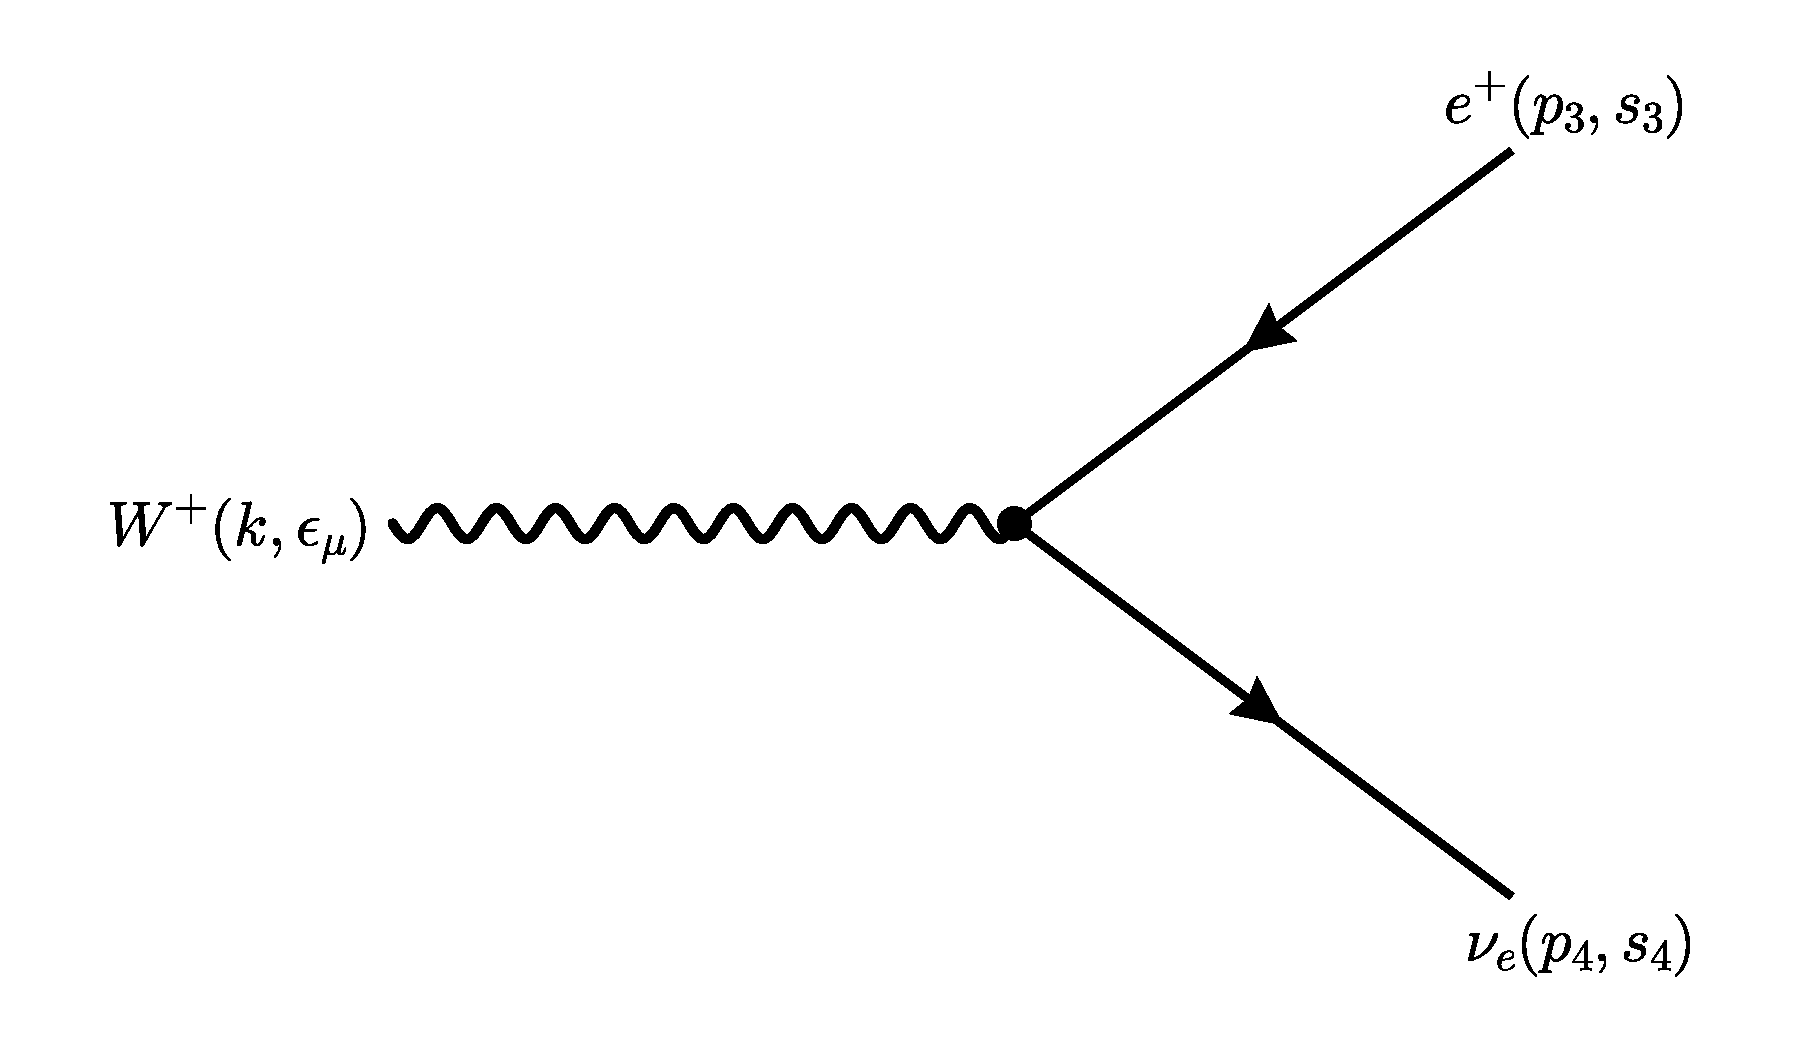
\includegraphics[width=0.6\linewidth]{graphics/W-decay-feyn}
	\caption{Feynman diagram representing the decay of $W^+$ to a positron and electron-neutrino.}
	\label{fig:w-decay-feyn}
\end{figure}

\underline{Feyman Rules}:
\begin{itemize}
	\item Following the fermion line backwards, the electron-neutrino is represented as a Dirac $\bar{u}$-spinor, where the bar corresponds to a four-component row vector, with four-momentum $p_4$ and spin $s_4$.
	\item The W$^+$  is represented as the vector boson current, $$-i\frac{g}{\sqrt{2}}\frac{1}{2}\gamma^\mu (1-\gamma^5)\epsilon_\mu(k, \lambda),$$ and one includes the polarisation vector, $\epsilon_\mu(k, \lambda)$, where $\lambda = 0, \pm1$ corresponds to the longitudinal and two transverse polarisation states of the W-boson and the momentum four-vector $k$.
	\item  The fermion line ends at the positron, which is represented as a Dirac $v$-spinor, which corresponds to a four-component column vector, with four-momentum $p_3$, mass $m_3$ and spin $s_3$.
\end{itemize}	
The amplitude, $\mathcal{M}$, is therefore: 

$$\mathcal{M} =\bar{u}(p_4, s_4) \left[-i \frac{g}{\sqrt{2}}\frac{1}{2}\gamma^\mu (1-\gamma^5) \epsilon_\mu (k, \lambda)\right] v(p_3, s_3),  $$

and then squaring gives,

$$ |\mathcal{M}|^2= |\mathcal{M}^*\mathcal{M}|= \frac{g^2}{2}\frac{1}{4}\left(\bar{u}(p_4, s_4) \left[\gamma^\mu (1-\gamma^5) \epsilon_\mu (k, \lambda)\right] v(p_3, s_3)\right)^*\left(\bar{u}(p_4, s_4) \left[\gamma^\nu (1-\gamma^5) \epsilon_\nu (k, \lambda)\right] v(p_3, s_3)\right). $$

The squared amplitude can be simplified by using the relation $\bar{u} = u^{\dagger}\gamma^0$ and the 
 from \ref{gamma_id}:

$$|\mathcal{M}|^2 = \frac{1}{4} \frac{g^2}{2} (\epsilon_\mu^* \bar{v}[\overline{\gamma^\mu (1-\gamma^5)}]u)(\bar{u}[\gamma^\nu (1-\gamma^5] v \epsilon_\nu). $$

 \subsection{Summing over lepton spin states}
 Once again, $\epsilon_{\mu}^*$ and $\epsilon_{\nu}$ will be treated separately later and will not contribute in the summation over spins. The notation for spin- and polarisation-summed amplitude squared will be split into the summation over spins component, denoted by $N^{\mu\nu}$, and summation over polarisation, denoted $Z_{\mu \nu}$, where, $$\sum_{s_3, s_4, \text{pol}}|\mathcal{M}|^2=  \frac{1}{4} \frac{g^2}{2} Z_{\mu\nu}N^{\mu\nu} $$\\
 
 Summing over the spin states of the electron-neutrino and positron can be done using the $v$-spinor and $u$-spinor completeness relations respectively \ref{completeness}. Using Casimir's trick, the spin summed component is given as,
 
 $$N^{\mu\nu}= 2\text{Tr}\left[\gamma^\mu (1-\gamma^5)(\slashed{p_4}-m_4)\gamma^\nu (1-\gamma^5) (\slashed{p_3}-m_3)\right],$$
 
 where the property \ref{overline-id} was used to convert $\overline{\gamma^\mu (1-\gamma^5)}$ back into $\gamma^\mu (1-\gamma^5).$ One can use the projector representation of $(1-\gamma^5)$ as $P_L = \frac{1}{2}(1-\gamma^5)$, and its properties to omit the mass terms in the expression, 
 
 \begin{equation}
 	\begin{aligned}
 		 N^{\mu\nu}&= 2\text{Tr}\left[\gamma^\mu (1-\gamma^5)\slashed{p_4}\gamma^\nu
 		\slashed{p_3}\right]\\
 		&= 2\text{Tr} \left[\gamma^\mu \slashed{p_4}\gamma^\nu \slashed{p_3}\right] - 2\text{Tr}\left[\gamma^\mu \gamma^5 \slashed{p_4}\gamma^\nu \slashed{p_3} \right]
 	\end{aligned}
 \end{equation}

  
 Evaluating the traces leads by using $ \text{Tr}[\slashed{p}\gamma^\mu \slashed{k} \gamma^\nu] = 4[p^\mu k^\nu + p^\nu k^\mu - (p \cdot k) g^{\mu \nu}]$ on the first term and $\text{Tr}[\gamma^\mu \gamma^\nu \gamma^\rho \gamma^\sigma \gamma^5] = -4i\epsilon^{\mu \nu \rho \sigma}$, the final expression of the spin summed component of the squared amplitude is,
 
 $$
 N^{\mu\nu}= 8[p_4^\mu p_3^\nu + p_4^\nu p_3^\mu - (p_3 \cdot p_4) g^{\mu \nu} -i \epsilon^{\mu \nu \rho \sigma}p_{3\rho}p_{4\sigma}].
 $$
 
 \subsection{Summing over initial polarisation states}\label{sum-over-initial-pol-states}
 In similar fashion to Section \ref{pol}, one can sum over the different initial polarisation states of the W-boson:
 \begin{equation}
 	Z_{\mu\nu}= \sum_\text{pol} \epsilon_\mu^* \epsilon_\nu=  -g_{\mu\nu} + \frac{k_\mu k_\nu}{M_W^2}.
 \end{equation}
The spin- and  polarisation-summed squared amplitude gives,

\begin{equation}
	\begin{aligned}
			\sum_{s_3, s_4, \text{pol}}|\mathcal{M}|^2&=  \frac{1}{4} \frac{g^2}{2} Z_{\mu\nu}N^{\mu\nu}\\
			&= \frac{1}{4} \frac{g^2}{2}   \left(-g_{\mu\nu} + \frac{k_\mu k_\nu}{M_W^2}\right) 8[p_4^\mu p_3^\nu + p_4^\nu p_3^\mu - (p_3 \cdot p_4) g^{\mu \nu} - i\epsilon^{\mu \nu \rho \sigma}p_{3\rho}p_{4\sigma}].
	\end{aligned}
\end{equation}
Contracting $g_{\mu \nu}$ with the terms in the square brackets gives,

\begin{equation}
	\begin{aligned}
		-8[p_{4\mu}p_3^\mu + p_{3\mu}p_4^\mu -4(p_3 \cdot p_4) -ig_{\mu\nu}\epsilon^{\mu \nu \rho \sigma}p_{3\rho}p_{4\sigma}] &= 8[-2(p_3 \cdot p_4) + 4(p_3 \cdot p_4)- 0] \\
		&= 16(p_3 \cdot p_4)
	\end{aligned}
\end{equation}
The contraction of $g_{\mu\nu}\epsilon^{\mu \nu \rho \sigma}p_{3\rho}p_{4\sigma}$ goes to zero because the Levi-Civita is totally antisymmetric and the metric tensor is symmetric under the exchange of indices. Contracting $\frac{k_\mu k_\nu}{M_W^2}$ gives, 

$$\frac{8}{M_W^2}[2(p_3 + p_4) \cdot p_4 (p_3 +p_4 )\cdot p_3 - (2p_3\cdot p_4)(p_3 \cdot p_4)]  = \frac{8}{M_W^2}[2(p_3 \cdot p_4)^2 - 2(p_3 \cdot p_4)^2] = 0.$$	
Therefore,

$$ \sum_{s_3, s_4, \text{pol}}|\mathcal{M}|^2=  \frac{1}{4} \frac{g^2}{2} Z_{\mu\nu}N^{\mu\nu} = \frac{1}{4} \frac{g^2}{2}  16(p_3 \cdot p_4) = 2g^2(p_3 \cdot p_4).$$

For the final step, $(p_3 \cdot p_4)$ can be expressed in terms of the Mandelstam variable, $s$. The Mandelstam variables are defined for a 2 $\rightarrow$ 2 scattering process; the decay of a W$^+$ boson is a 1 $\rightarrow$ 2 process. However, one can still use the variable $s = (p_3 + p_4)^2 = k^2$. Assuming that the $e^+$ and $\nu_e$ are massless, $s = 2(p_3 \cdot p_4) =k^2$, and due to the on-shell condition, $k^2 = M_W^2$. Thus, 
\begin{equation}
	 \sum_{s_1, s_2, \text{pol}}|\mathcal{M}|^2 = \frac{1}{3}g^2 M_W^2,	
\end{equation}
where the factor of 1/3 came from averaging over initial polarisation states for $W^+.$




\subsection{Calculating decay rates}
One can derive the differential decay rate, $d \Gamma$, via a small modification to the general expression of the differential cross-section (Eq. \ref{general_cross}). Specifically, one can remove factors that involve a multi-particle initial state; the decaying $W^+$ boson is assumed to be at rest, so the factor 1/E$_A$ becomes 1/$M_W$. Thus the differential decay rate formula is,

\begin{equation}
	d\Gamma= \frac{|\mathcal{M}|^2 }{2M_W} d\Phi_{n_f},
\end{equation}
where,

$$ d\Phi_{n_f}=	 \left(\prod_{f}^{N_f}\frac{d^3\boldsymbol{p}_f}{(2\pi)^32E_f}\right) (2\pi)^4 \delta^4 (p_A - \Sigma p_f),$$

is the Lorentz-invariant phase space factor, $N_f$ is the number of final state particles, $p_f$ is the momenta of the final state particle and $m_A$ is the mass of the initial (decaying) particle. Hence the differential decay rate in the $W^+$ rest frame is,

\begin{equation}
	d\Gamma (W^+ \rightarrow e^+ \nu_e) =  \frac{1}{2M_W} \left(\frac{1}{3}g^2 M_W^2\right) d\Phi_{2}.
\end{equation}

Working out the phase space integral is straightforward. 

\begin{equation}
	\begin{aligned}
		d\Phi_{2}&=	 \left(\frac{d^3\boldsymbol{p}_e d^3\boldsymbol{p}_\nu}{4(2\pi)^6E_eE_\nu}\right) (2\pi)^4 \delta^4 (p_W -  p_e - p_\nu) \\
		&= \left(\frac{d^3\boldsymbol{p}_e d^3\boldsymbol{p}_\nu}{4(2\pi)^6E_eE_\nu}\right) (2\pi)^4 \delta(M_W - E_e - E_\nu)\delta^3 (\boldsymbol{p}_W -  \boldsymbol{p}_e - \boldsymbol{p}_\nu),
	\end{aligned}
\end{equation}
where the 4-dimensional delta function is split into 1-dimensional energy and 3-dimensional momentum components. Since the W$^+$ is assumed to be at rest, $E_W = M_W$.


$$
\int d\Phi_{2} =  \frac{1}{4} \frac{1}{(2\pi)^2}\int  \left(\frac{d^3\boldsymbol{p}_e d^3\boldsymbol{p}_\nu}{E_eE_\nu}\right) \delta(M_W - E_e - E_\nu)\delta^3 (\boldsymbol{p}_W -  \boldsymbol{p}_e - \boldsymbol{p}_\nu).
$$
One can assume the masses of the positron and electron neutrino to be zero; this is justified as $m_e, m_\nu << M_W$. Thus, $E_e = |\boldsymbol{p_e}| $ and $E_\nu = |\boldsymbol{p}_\nu| $. Since the $W^+$ is assumed to be at rest, it is trivially the center-of-mass frame, so $\boldsymbol{p}_e = - \boldsymbol{p}_\nu$,  and so it follows that $E_e = E_\nu= E^*$. One can do the  $d^3\boldsymbol{p}_\nu$ integral using $\delta^3 (\boldsymbol{p}_W -  \boldsymbol{p}_e - \boldsymbol{p}_\nu)$, 
% i think here, you integrate momentum of nu using delta function to fix the moomentum of nu 
$$
\int d^3\boldsymbol{p}_2\; \delta^3 (\boldsymbol{p}_W -  \boldsymbol{p}_e - \boldsymbol{p}_\nu) = 1,
$$
which gives,
$$
\int d\Phi_{2} = \frac{1}{4} \frac{1}{(2\pi)^2} \int  \left(\frac{d^3\boldsymbol{p}_e}{E^{*2}}\right)\delta(M_W - 2|\boldsymbol{p}_e|),
$$
where $-E_e - E_\nu= -|\boldsymbol{p}_e|-|\boldsymbol{p}_e| = -2|\boldsymbol{p}_e|$.
One can work in spherical coordinates, where $d^3 \boldsymbol{p}_e = |\boldsymbol{p}_e|^2 d|\boldsymbol{p}_e| d\Omega$, where $d\Omega = \sin\theta d\theta d\phi$. Omitting the prefactor for now and changing to spherical coordinates gives, 

\begin{equation}
	\int \left(\frac{1}{E^{*2}}\right) |\boldsymbol{p}_e|^2 d|\boldsymbol{p}_e| d\Omega \; \delta(M_W - 2|\boldsymbol{p}_e|).
\end{equation}


Since $|\boldsymbol{p}_e|^2 = E^{*2}$, the factor $|\boldsymbol{p}_e|^2/E^{*2} =1$:

$$
\int  d|\boldsymbol{p}_e|\delta(M_W - 2|\boldsymbol{p}_e|) \int d\Omega.
$$
In Section \ref{sum-over-initial-pol-states}, the initial polarisation states of the W$^+$ was summed and averaged over which removes any preferred spin direction. If one worked in a frame where $\boldsymbol{p}_W \neq 0$, the momentum vector of the W$^+$ defines an axis of motion; decay products can be boosted along that axis, thus the angular distribution depends on the angle relative to $\boldsymbol{\hat{p}}_W$. It was assumed that the W$^+$ decays at rest, therefore, this calculation will work in the frame in which the decays have rotational symmetry, thus are isotropic. Integrating over the full solid angle gives,

$$
\int d\Omega = 4\pi.
$$
In order to do the $d|\boldsymbol{p}_e|$ integral, one needs to get the $2|\boldsymbol{p}_e|$ term in the delta function, $\delta(M_W - 2|\boldsymbol{p}_e|)$,  to match the integration variable $|\boldsymbol{p}_e|$. This is so that one can use,


$$
\int dx \; \delta(x) = 1.
$$

This can be accomplished through the property,

$$
	\delta(f(x))
=
\sum_{j=1}^{n}
\frac{\delta(x-x_j)}{\bigl| f'(x_j) \bigr|},
\qquad
\text{for $n$ simple roots of f(x)}.
$$
 
Here, $f(x) = f(\boldsymbol{p}_e) = M_W - 2|\boldsymbol{p}_e|$ and has a simple root at $|\boldsymbol{p}_e| = M_W/2.  $ The first derivative of $f(\boldsymbol{p}_e) = -2$. The delta function becomes:

$$
\delta(M_W -2|\boldsymbol{p}_e|) = \frac{\delta(\boldsymbol{p}_e - M_W/2)}{2}.
$$ 
The remaining integral is therefore,

$$
\frac{1}{2}\int  d|\boldsymbol{p}_e| \delta(\boldsymbol{p}_e - M_W/2) = \frac{1}{2}.
$$
Putting all the factors back together, the integrated phase space factor is

$$
\int d\Phi_{2} =  \frac{1}{4} \frac{4\pi}{(2\pi)^2} \frac{1}{2} = \frac{1}{8\pi},
$$
 which leads to the partial decay width,
 
 \begin{equation}
 	\Gamma(W^+ \rightarrow e^+ \nu_e)= \frac{1}{48}g^2M_W = \frac{G_F}{\sqrt{2}}\frac{M_W^3}{6\pi}.
 \end{equation}

For $M_W = 80.369$ GeV \cite{CMS:2024lrd}, the numerical value of this partial decay width is,

$$
\Gamma(W^+ \rightarrow e^+ \nu_e) = 0.227\; \text{GeV} = \Gamma^0_W.
$$

\subsection{$W^+ \rightarrow e^+ \nu_e$ branching ratio calculation}
Assuming all quark-antiquark decays eventually fragment to hadrons, one can do an inclusive calculation where the total hadronic decay rate is the approximated by the quark-antiquark decay rate. In the massless fermion approximation, it is justified for the tree-level partial decay widths of $\mu$, $\tau$ leptons and quarks to be identical, where the quark channels differ up to a colour and CKM factor:

$$
\Gamma(W^+ \rightarrow e^+ \nu_e) = \Gamma(W^+ \rightarrow \mu^+  \nu_\mu) = \Gamma(W^+  \rightarrow \tau^+  \nu_\tau) = \Gamma^0_W 
$$
and, 

$$ \Gamma(W^+ \rightarrow q\bar{q}) = 3 |V_{q\bar{q}}|^2 \Gamma^0_W,$$

where the factor of 3 comes from summing the three colours. For the kinematically accessible decays, one can use CKM unitarity where,

$$
\sum_{q\bar{q}} |V_{q\bar{q}}|^2 = 2, 
$$
where $q = u,c$ and $\bar{q} = d, s, b$. The specific contributions are,

\begin{equation*}
	\begin{align}
	|V_{ud}|^2 + |V_{us}|^2 +|V_{ub}|^2  =1\\
	|V_{cd}|^2 + |V_{cs}|^2 +|V_{cb}|^2  =1, 	
	\end{align}
\end{equation*}
which would give a value of $\Gamma(W \rightarrow q\bar{q}) = 6\Gamma^0_W$. The naive contribution would include decays into top-quark and corresponding down-type quarks. Therefore the total decay width is, 

$$
\Gamma(W^+ \rightarrow \text{all}) \simeq \Gamma(W^+ \rightarrow \text{hadrons}) + \Gamma(W^+ \rightarrow \text{leptons}) \simeq 6\Gamma^0_W + 3\Gamma^0_W \simeq 9\Gamma^0_W = 2.025\; \text{GeV}.
$$
Including contributions from $W^+$ decays into top-quarks increases the total decay width to $2.7$ GeV. Given that 1 GeV $= 1.52 \cross 10^{24} s^{-1}$, the mean lifetime of  $W^+$ is $\tau = 1/\Gamma \simeq 3.249 \cross 10^{-25} s$. The branching ratio of $W^+$ decaying into $e^+ \nu_e$ is given as,

\begin{equation}
	BR(W \rightarrow e^+ \nu_e) \simeq \frac{\Gamma(W^+ \rightarrow e^+ \nu_e) }{\Gamma(W^+ \rightarrow \text{all})} = \frac{1}{9}
\end{equation}

\subsection{Obtaining total cross-section $\sigma(pp \rightarrow W^+ \rightarrow e^+ \nu_e)$ using NWA}

To obtain the observable rate for the leptonic final state we multiply the inclusive hadronic production cross section for an on-shell W$^+$ by the branching ratio for the decay $W^+ \rightarrow e^+ \nu_e$ . Under the  narrow-width approximation the production and decay factorise: production sets the number of on-shell W$^+$ bosons, and the branching ratio gives the fraction of those that decay to the chosen channel. Hence the total cross section for producing an $e^+ \nu_e$ final state is,

$$
	\sigma(pp \rightarrow W^+ \rightarrow e^+ \nu_e) = 	\sigma(pp \rightarrow W^+) \cross BR(W \rightarrow e^+ \nu_e).
$$
This relation is valid only if: the total width of W$^+$ is smaller that its mass ($\Gamma \ll M_W$); the daughter particles are much less massive than the parent ($m_{e^+}, m_{\nu_e} \ll M_W$); the scattering energy is much larger than the $M_W$, ($\sqrt{s} \gg M_W$); there is no significant interference with non-resonant processes; and the resonant propagator is separable from the matrix element \cite{Berdine:2007uv}. One gets the total hadronic cross-section at $\sqrt{s} = 13$ TeV as,

\begin{equation}
		\sigma(pp \rightarrow W^+ \rightarrow e^+ \nu_e) = 	0.7085 \pm 0.0042\; \text{nb} \cross \frac{1}{9} = 0.0787 \pm 0.0004\; \text{nb},
\end{equation}
and for a proton-anti-proton collision, 
\begin{equation}
	\sigma(p\bar{p} \rightarrow W^+ \rightarrow e^+ \nu_e) = 0.9068 \pm 0.0033\; \text{nb} \cross \frac{1}{9} = 0.1008 \pm 0.0004\; \text{nb}.
\end{equation}

\appendix
\section{Numerical integration code}
\subsection{Integration via \texttt{SciPy}}\label{integration-scipy}
\begin{minted}
[
frame=lines,
framesep=1mm,
baselinestretch=1.0,
bgcolor=LightGray,
fontsize=\scriptsize,
linenos
]
{python}
import lhapdf
import scipy.integrate as integrate
import math

pdf = lhapdf.mkPDF("PDF4LHC21_40", 0) #importing the PDF set

#constants
MW = 80.379
GF = 1.1663787e-5 
s = (13000)**2 #for a 13 TeV collider
tau = MW**2/s

prefactor= ((math.pi*math.sqrt(2))/2) * GF * MW * (1/s)


crssctn, error = integrate.quad(
lambda x1: prefactor * 1/x1 * (pdf.xfxQ(2, x1, MW))/x1 * (pdf.xfxQ(-1, tau/x1, MW))/ (tau/x1), tau, 1.0

)
# scipy.integrate.quad() has two outputs in the form: value, err.
#   -  quad() has args (func, a, b). 

# arg of xfxQ looks like: (id: PDG Parton id, x: momentum fraction, q: energy/ renormalisation scale)
#   -  id, https://pdg.lbl.gov/2022/reviews/rpp2022-rev-monte-carlo-numbering.pdf   
#   -  q, LHAPDF squares internally, hence MW not MW**2


print(f'{crssctn * 0.389379 * 1e6} ± {error * 0.389379 * 1e6} nb' )

# 1 GeV^-2 = 0.389379 mb 
\end{minted}
\subsection{Basic Monte Carlo Integration}\label{basic-mc-integration}
\begin{minted}
		[
	frame=lines,
	framesep=1mm,
	baselinestretch=1.0,
	bgcolor=LightGray,
	fontsize=\scriptsize,
	linenos
	]
	{python}
	
	import numpy as np 
	import lhapdf
	import math
	
	pdf = lhapdf.mkPDF("PDF4LHC21_40", 0) #importing the PDF set
	
	#constants
	MW = 80.379
	GF = 1.1663787e-5 
	s = (13000)**2 #for a 13 TeV collider
	tau = MW**2/s
	
	prefactor= ((math.pi*math.sqrt(2))/2) * GF * MW * (1/s)
	
	f= lambda x1: prefactor * 1/x1 * (pdf.xfxQ(2, x1, MW))/x1 * (pdf.xfxQ(-1, tau/x1, MW))/ (tau/x1)
	rand = np.random.uniform(tau, 1, 1000) #generate a 1000 length array of random numbers from tau to 1
	rand_comp = np.array([f(x1) for x1 in rand])
	#loops over every entry in the rand array, feeds them into pdf.xfxQ, and creates an array of the output
	est= (1-tau)*rand_comp.mean()
	#lhapdf function only itakes 0-Dim arrays i.e. a single value
	
	err = (1 - tau) * rand_comp.std(ddof=1) /np.sqrt(len(rand))
	# rand_comp.std(ddof=1) is the SD of the evaluated points
	
	
	print(f'cross-section: {est * 0.389379 * 1e6} ± {err* 0.389379 * 1e6} nb')
\end{minted}


\subsection{Integration via \texttt{VEGAS}}\label{integration-vegas}
\begin{minted}
	[
	frame=lines,
	framesep=1mm,
	baselinestretch=1.0,
	bgcolor=LightGray,
	fontsize=\scriptsize,
	linenos
	]
	{python}

import lhapdf
import math
import vegas

pdf = lhapdf.mkPDF("PDF4LHC21_40", 0) #importing the PDF set

#constants
MW = 80.379
GF = 1.1663787e-5 
s = (13000)**2 #for a 13 TeV collider
tau = MW**2/s

prefactor= ((math.pi*math.sqrt(2))/2) * GF * MW * (1/s)


f = lambda x: prefactor * 1/x[0] * (pdf.xfxQ(2, x[0], MW))/x[0] * (pdf.xfxQ(-1, tau/x[0], MW))/ (tau/x[0])

# VEGAS passes a list/array, even for 1D integrals i.e. x = [0.234]; this format is useful for multi-D integrals
# where x = [0.212, 0.111, 0.442,...]

# The list contains all the randomly sampled points per integration variable.
# but LHAPDF pdf.xfxQ() expects a float.
# Solution: x_1 --> x[0] (for 1D intgration) which extracts the first element of the list (a float) and passes 
# that into LHAPDF.

integ = vegas.Integrator([[tau, 1.0]])  # single variable x1
result = integ(f, nitn=10, neval=1000)  # 10 iterations, 1000 evaluations per iteration

print(result.summary())

print(f'result = {result* 0.389379 * 1e6} ± {result.sdev  * 0.389379 * 1e6} nb')
\end{minted}



































\bibliographystyle{unsrt}


\bibliography{major-project-bibliography}






\end{document}